%!TEX root = ../../report.tex
\begin{appendices}
    \section{Profile selection}
    \label{app:profile_selection}
        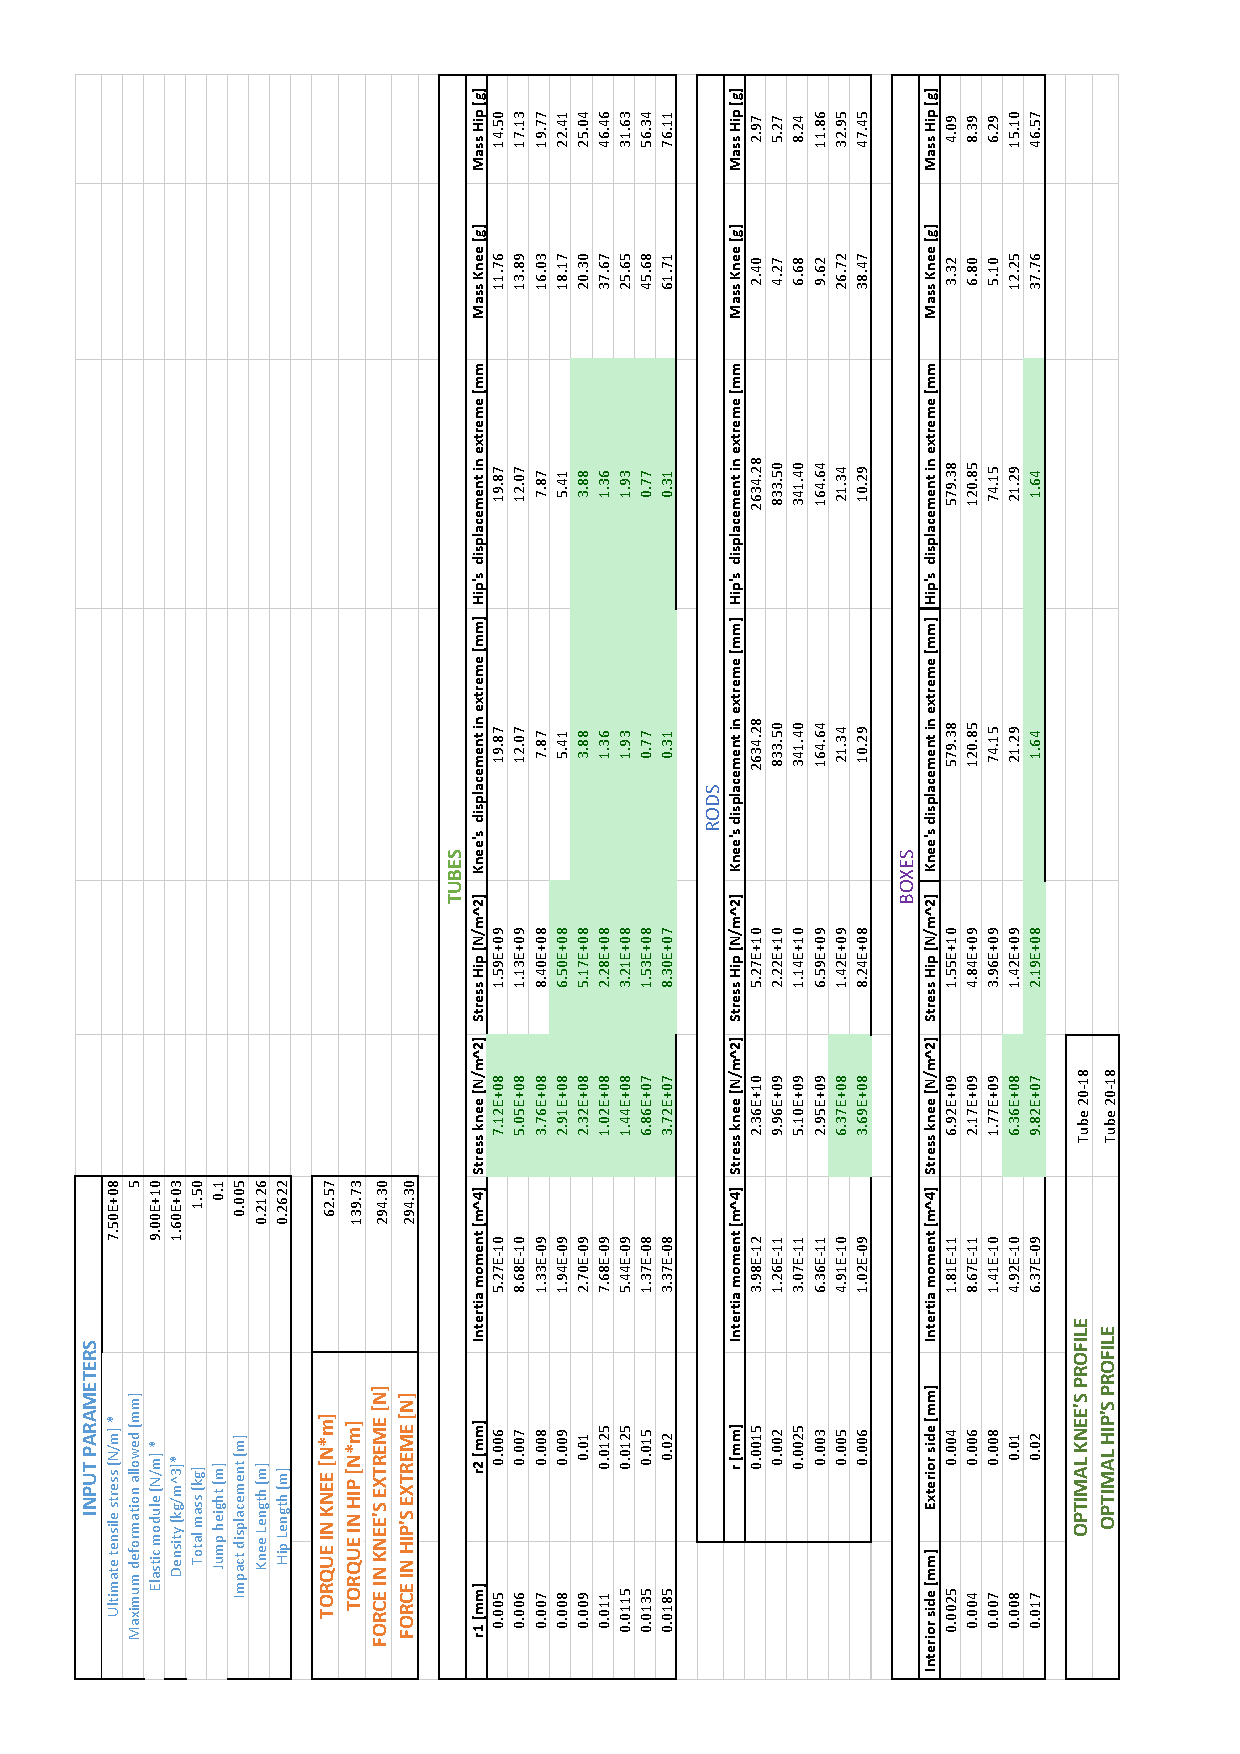
\includegraphics[width=177mm]{chapters/cha_appendices/profile_selection}

    \section{Mechanical drawings}
    \label{app:mechanical_drawings}
        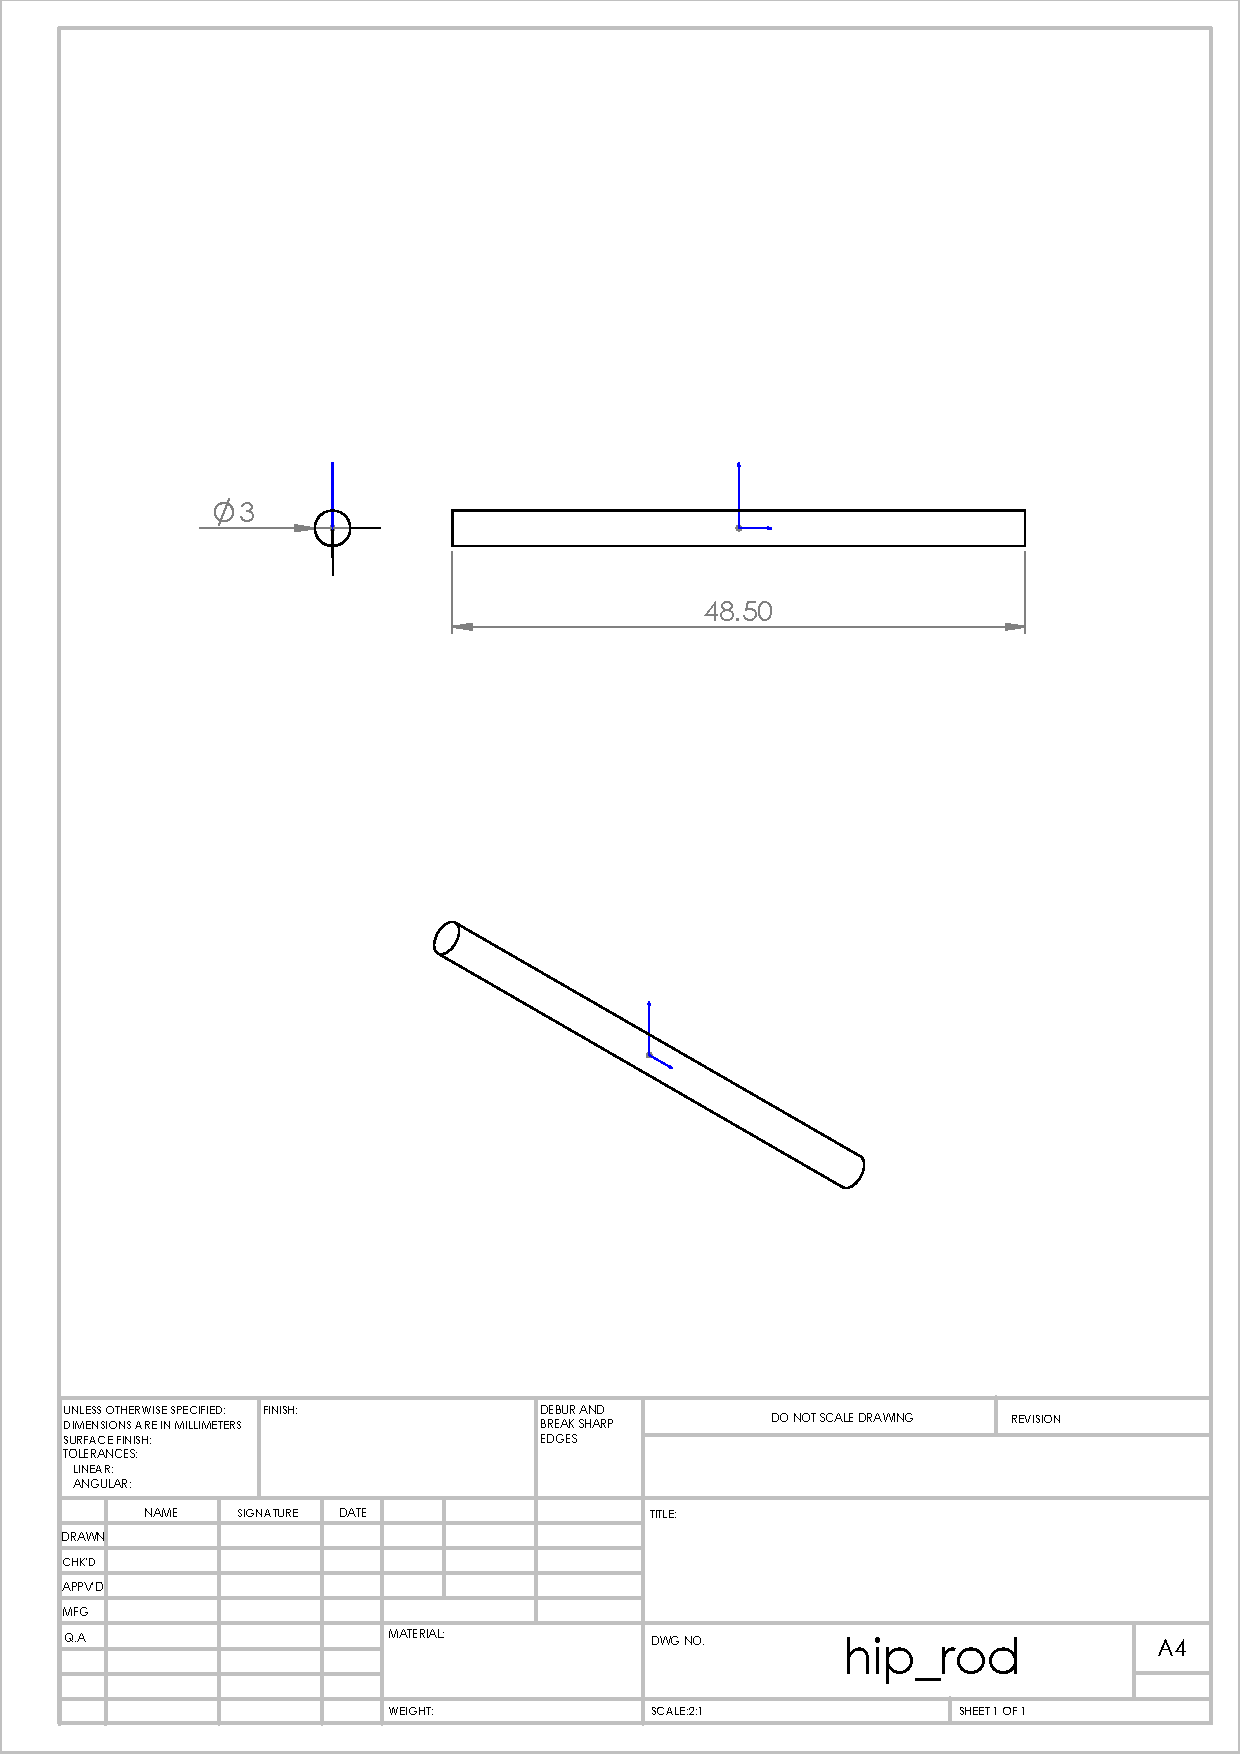
\includegraphics[width=\linewidth]{chapters/cha_appendices/hip_rod}
        \break
        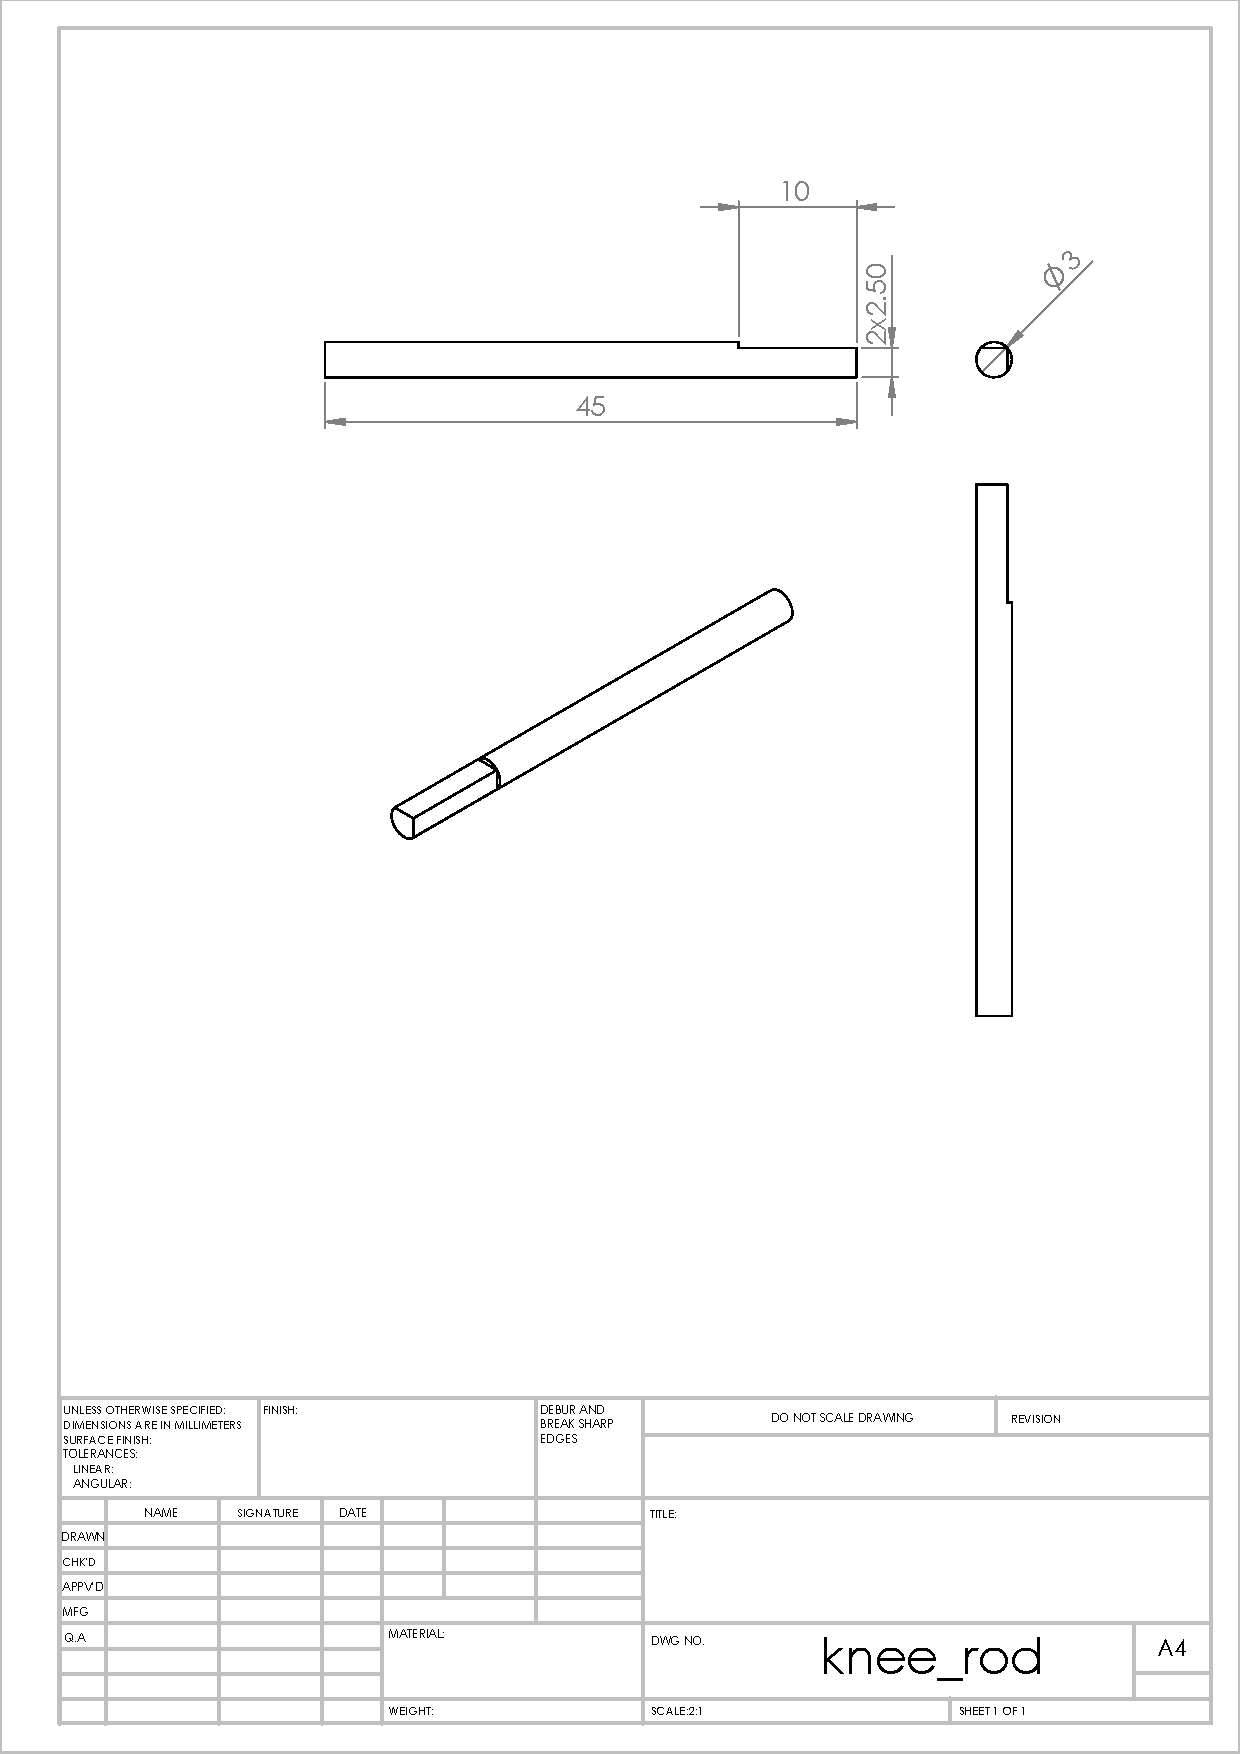
\includegraphics[width=\linewidth]{chapters/cha_appendices/knee_rod}
        \break
        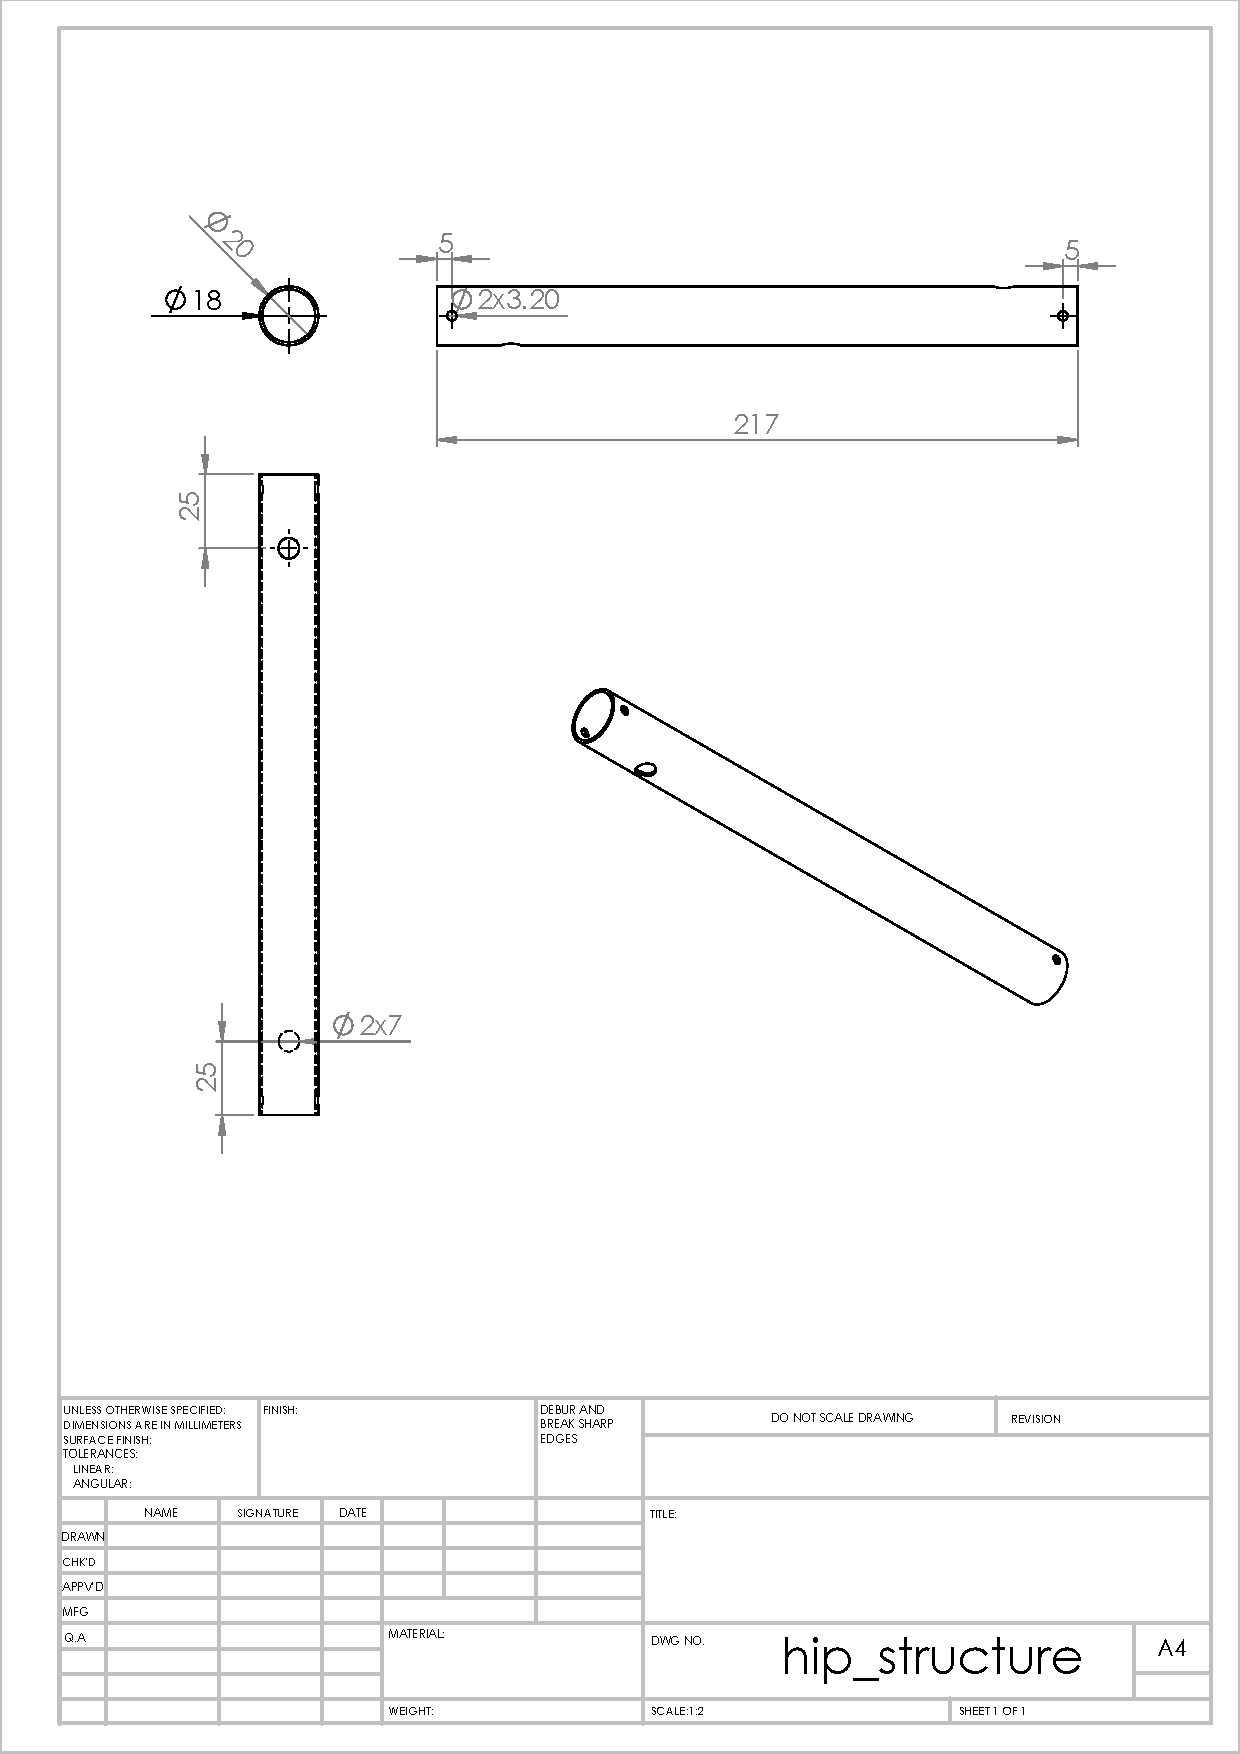
\includegraphics[width=\linewidth]{chapters/cha_appendices/hip_structure}
        \break
        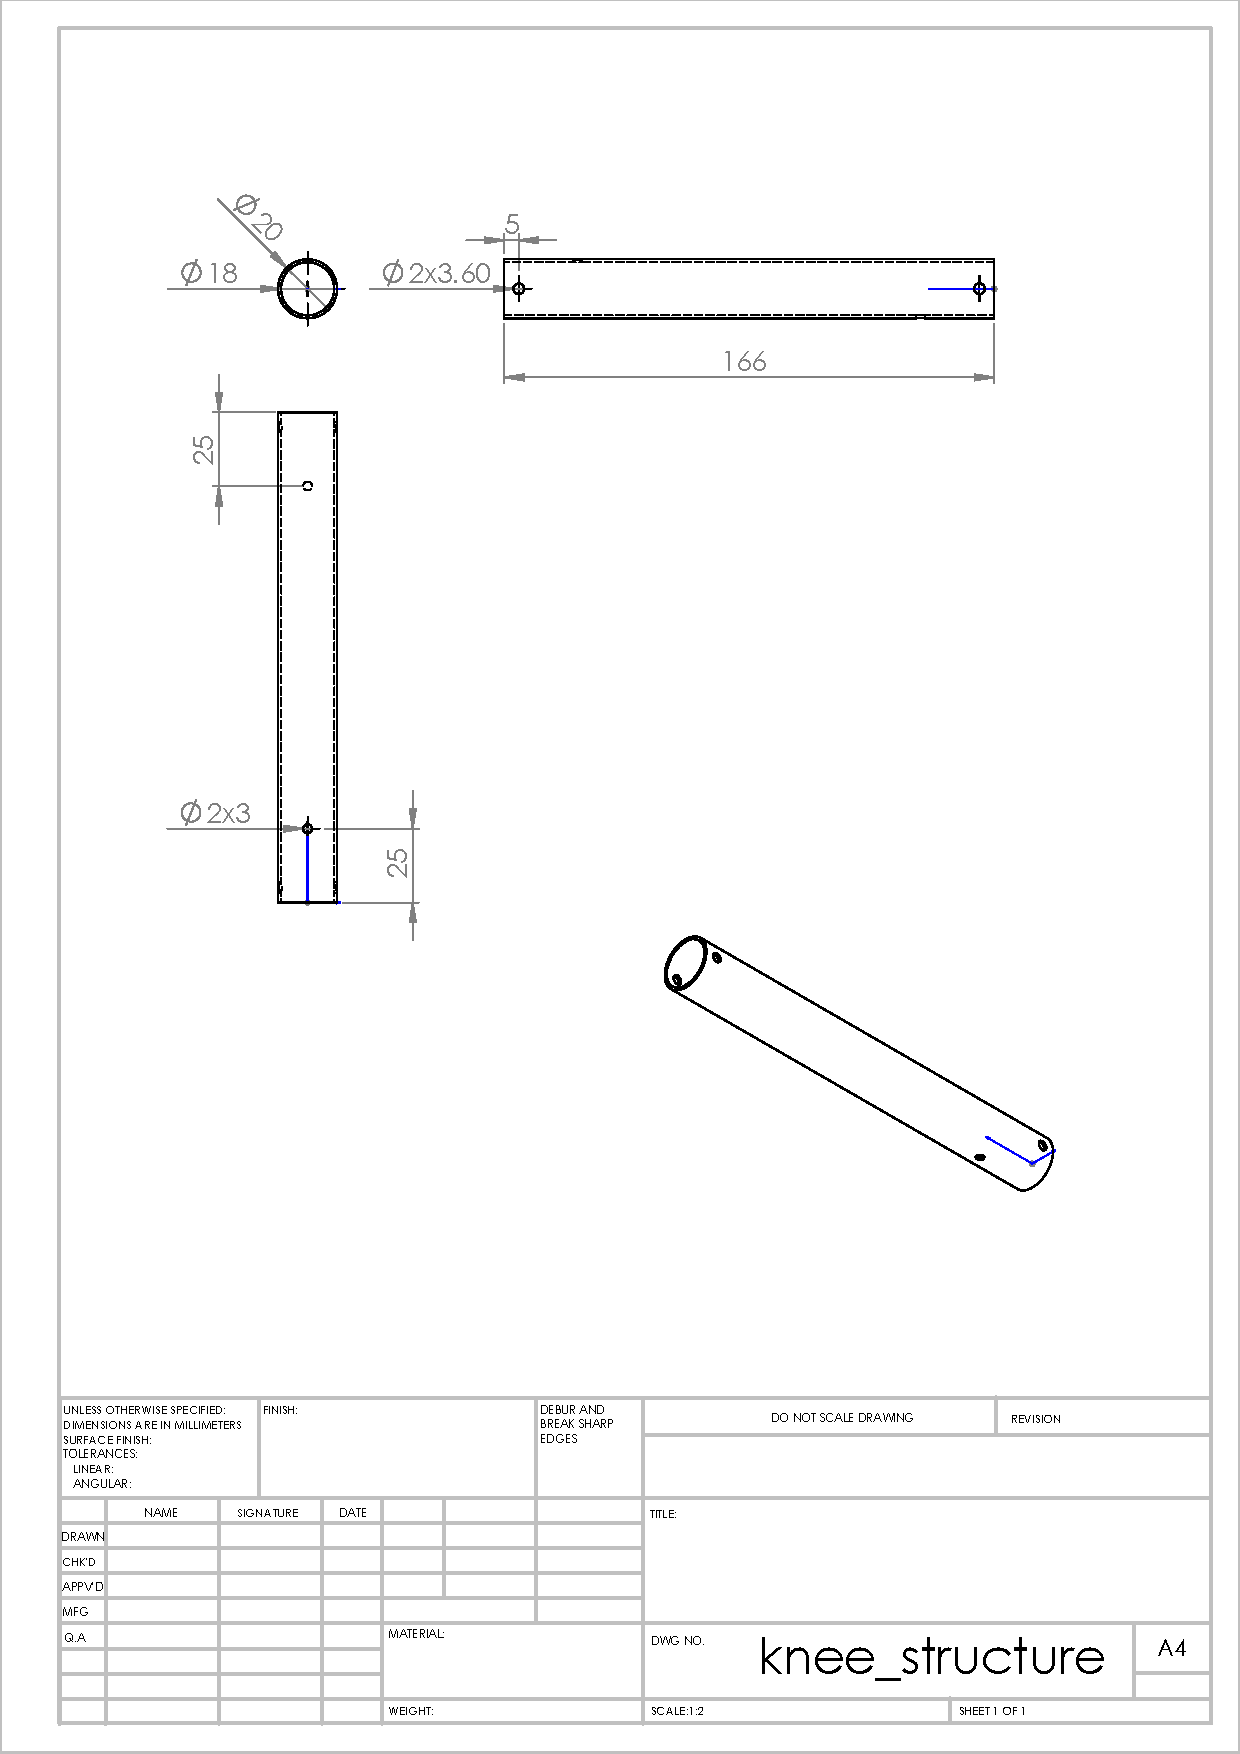
\includegraphics[width=\linewidth]{chapters/cha_appendices/knee_structure}
        \break
        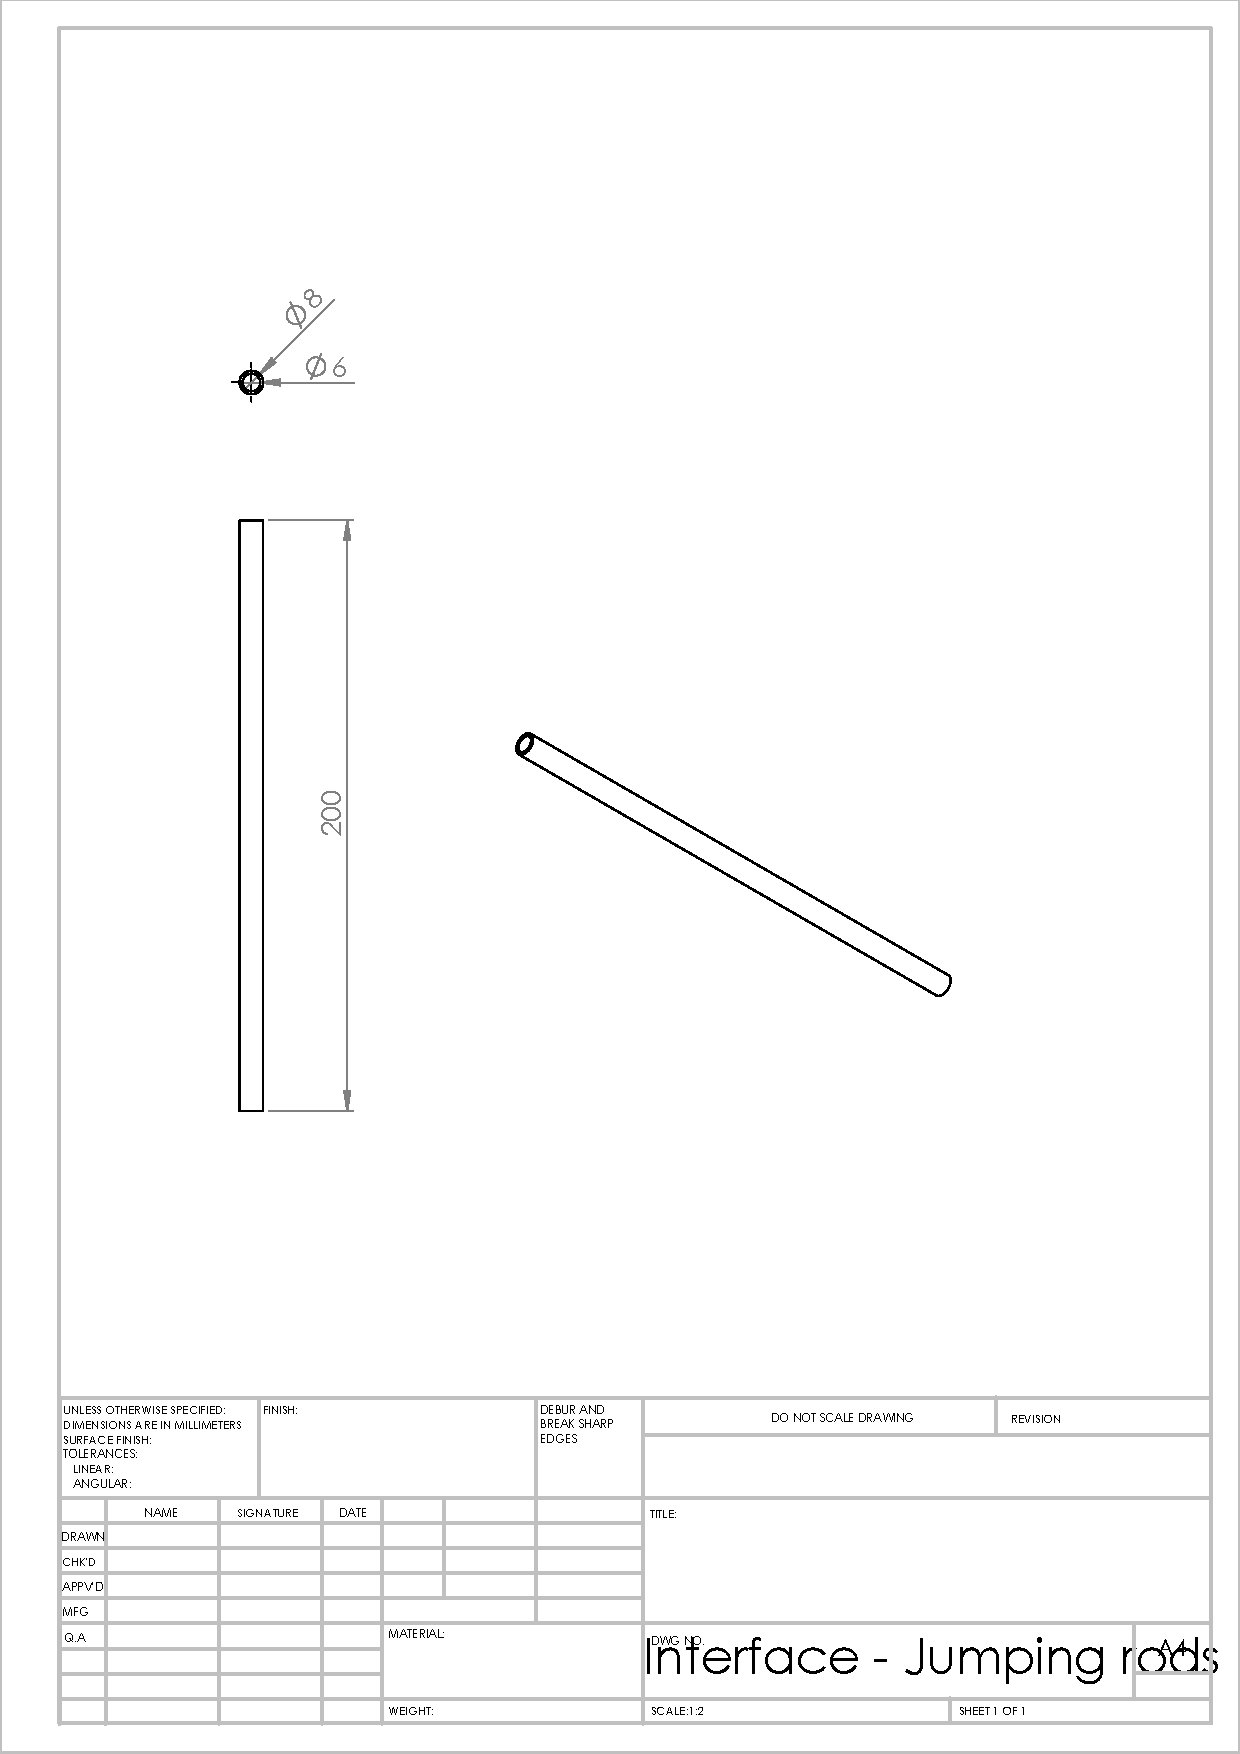
\includegraphics[width=\linewidth]{chapters/cha_appendices/interface_jumping_rods}
        \break
        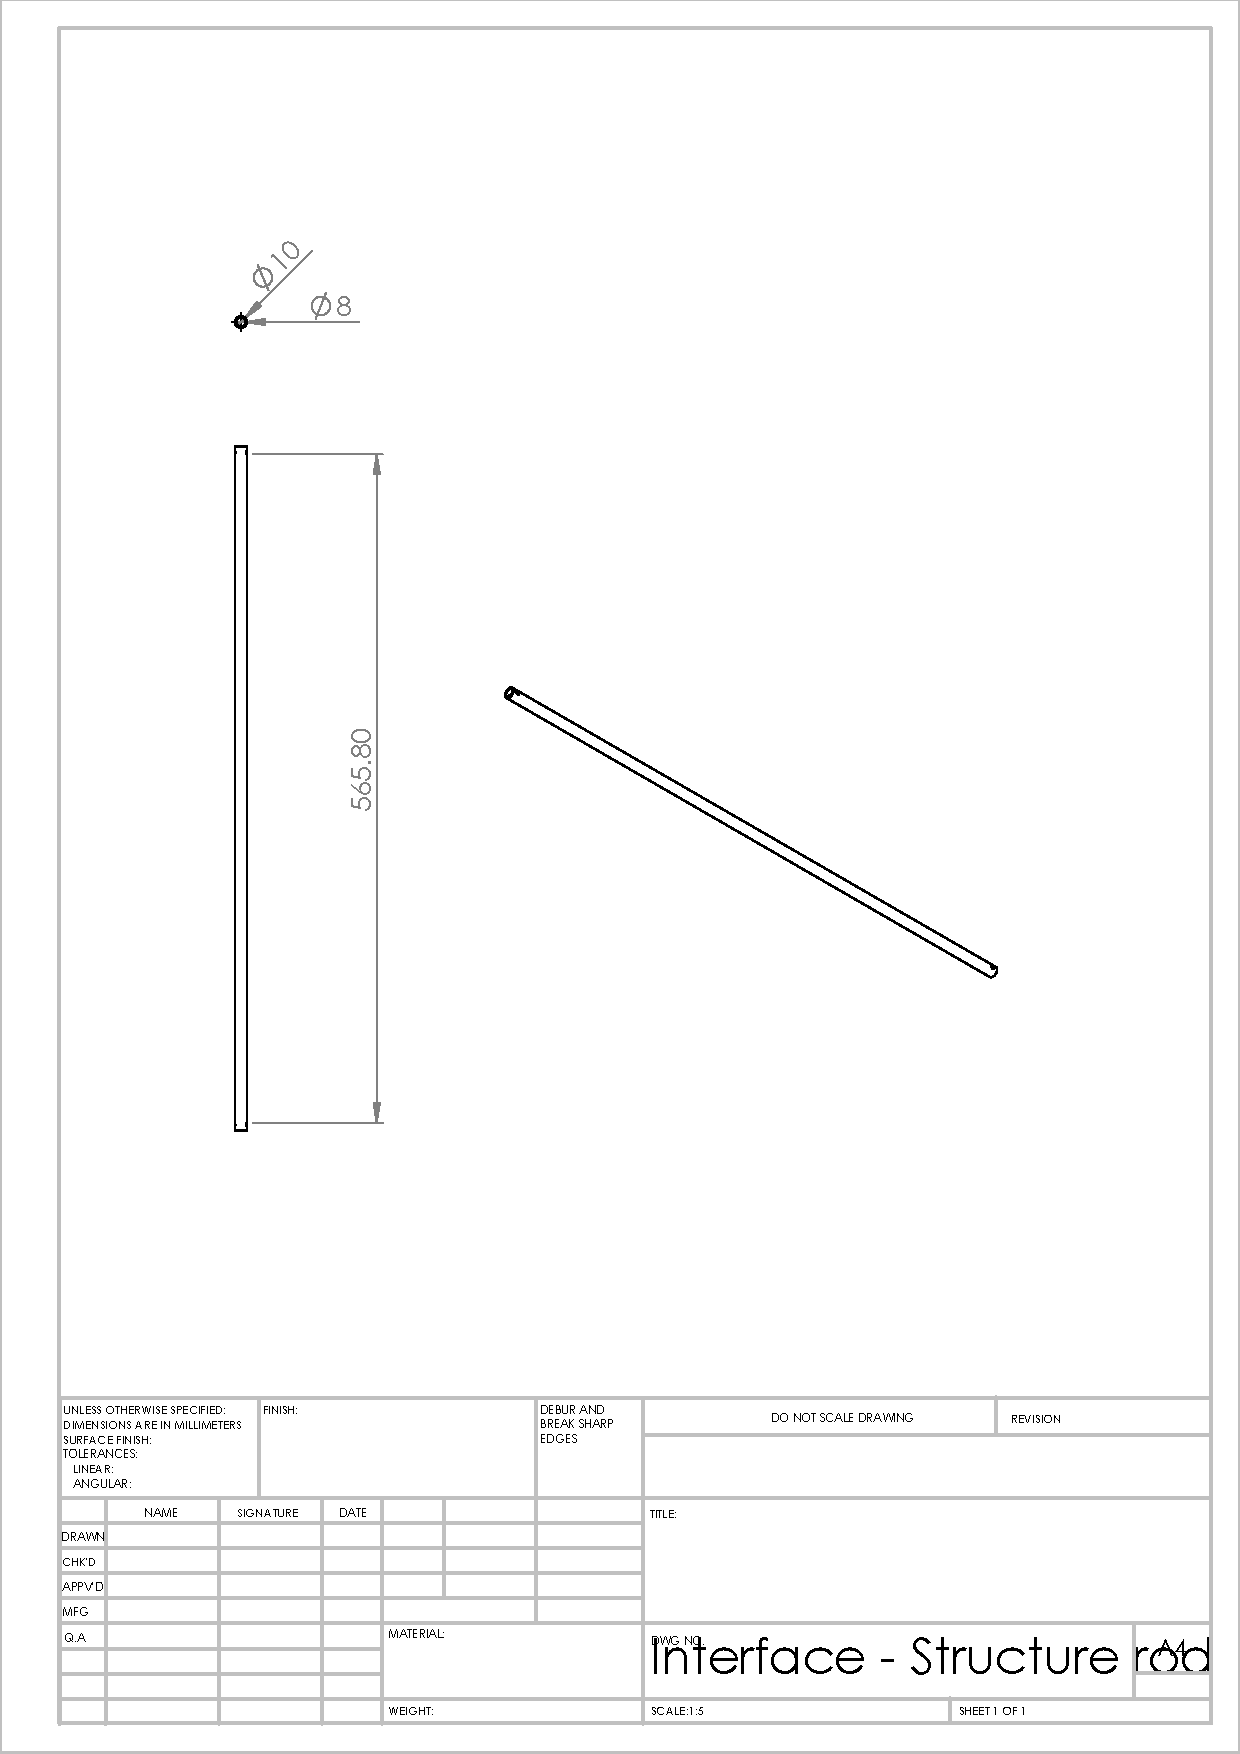
\includegraphics[width=\linewidth]{chapters/cha_appendices/interface_tructure_rod}
        \break
        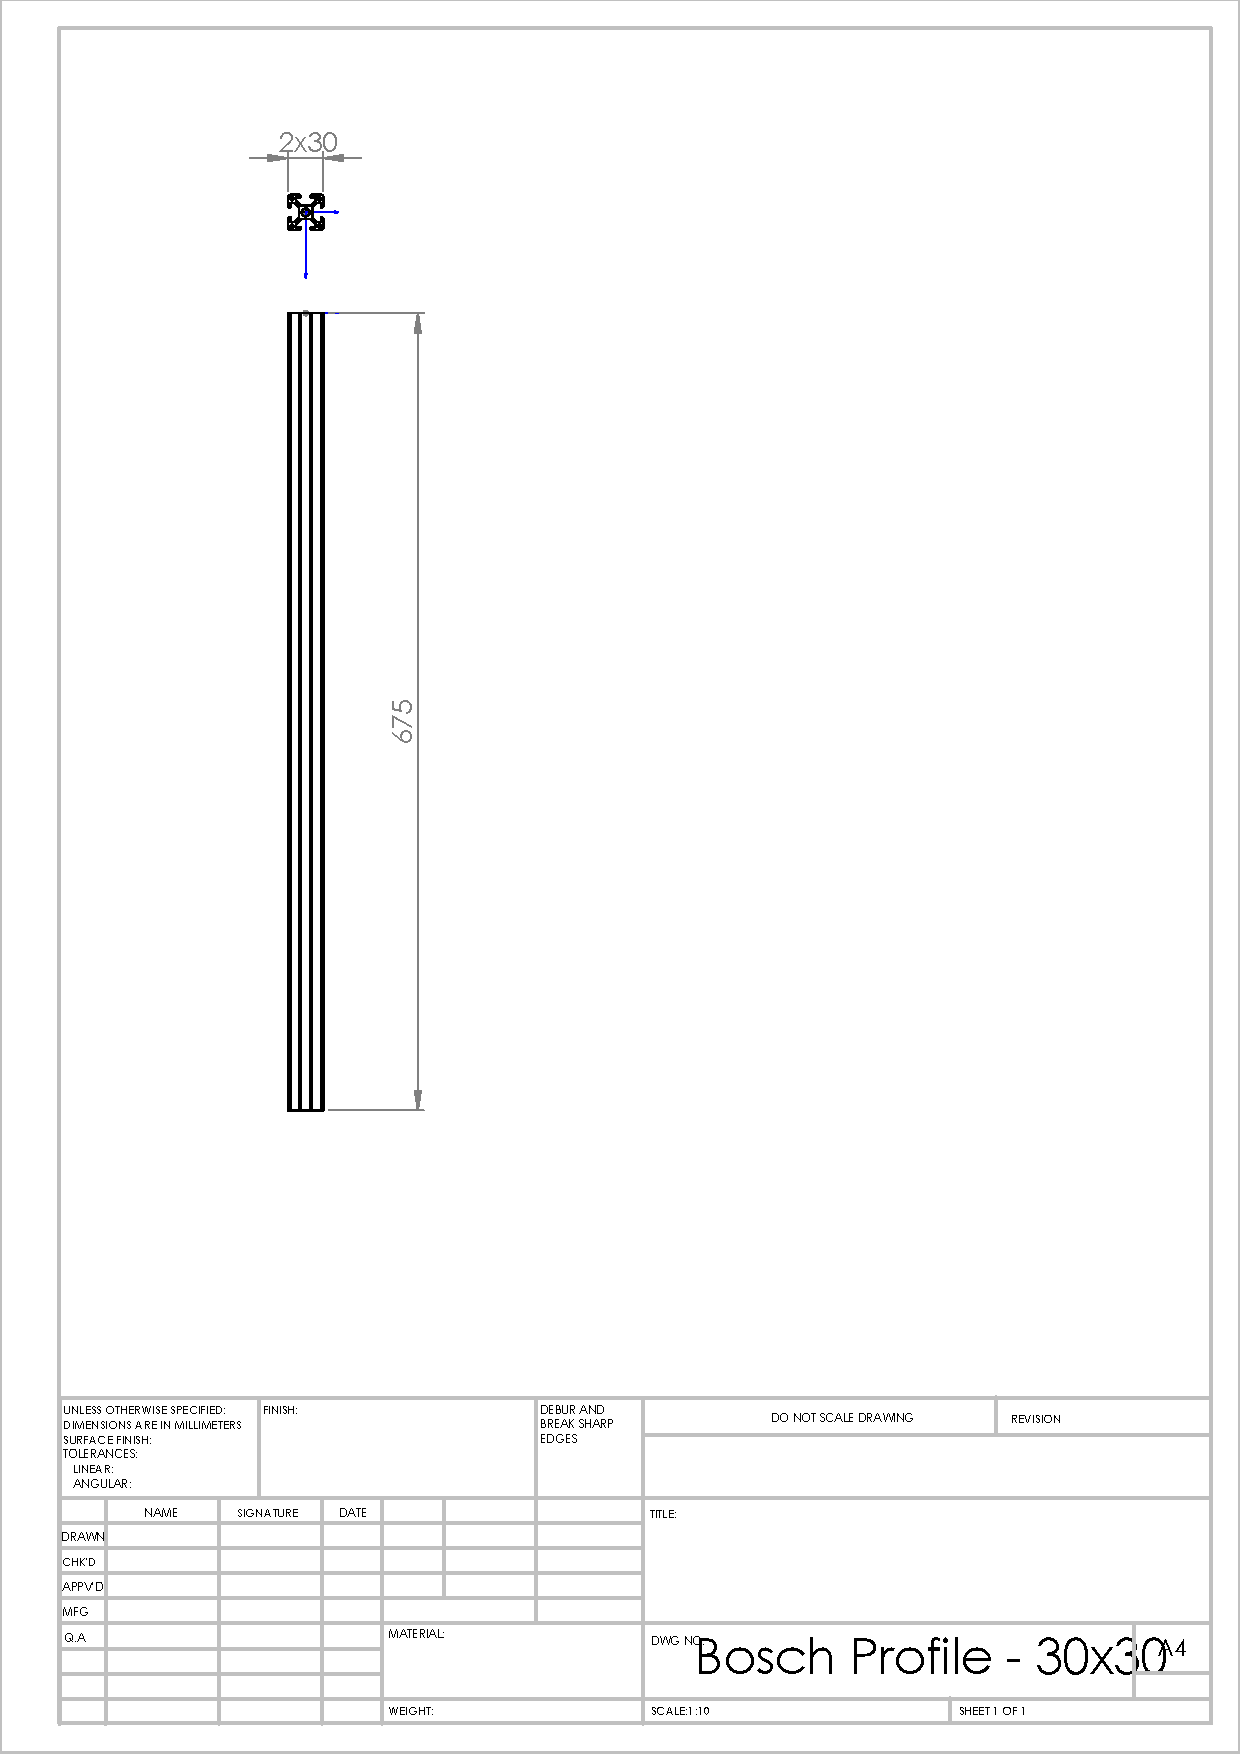
\includegraphics[width=\linewidth]{chapters/cha_appendices/bosch_profile}

    \section{CAD parameters}
    \label{app:cad_parameters}
        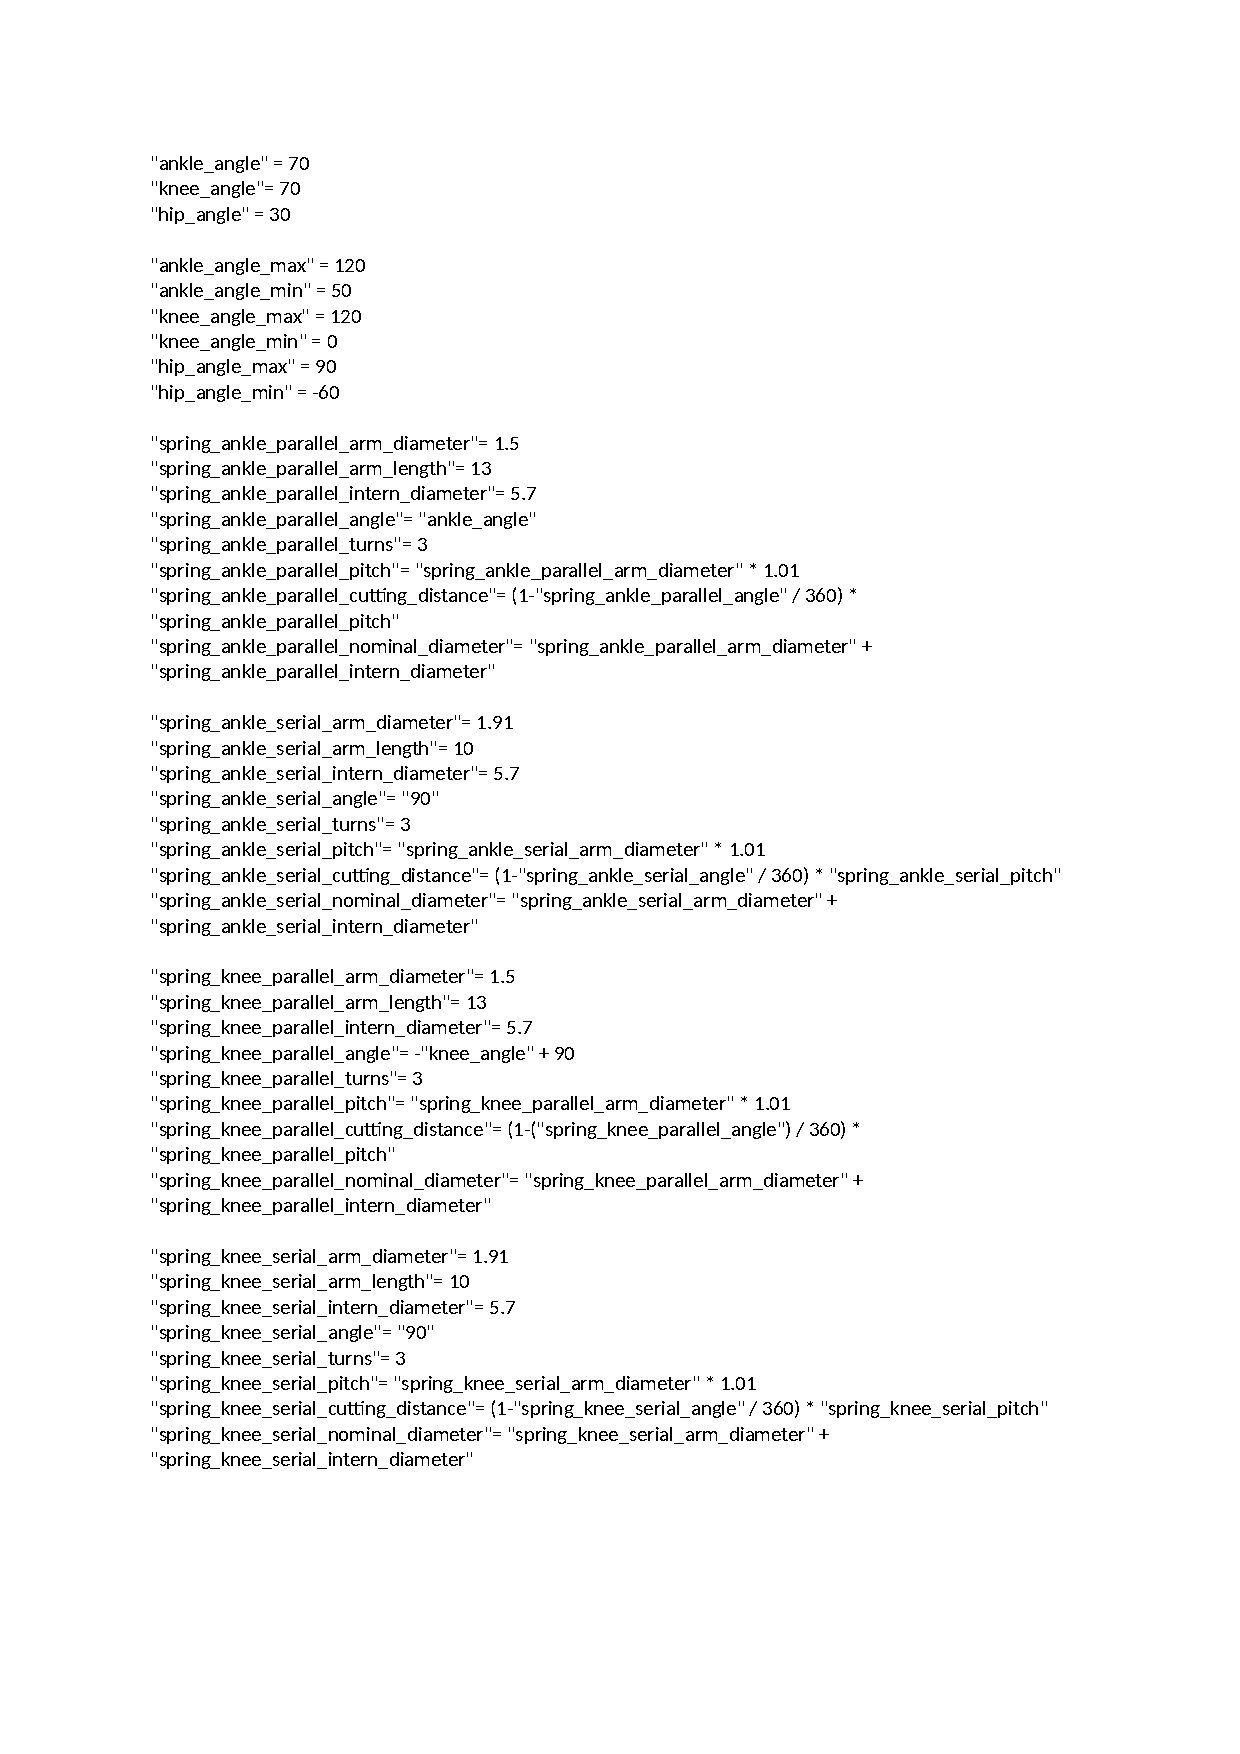
\includegraphics[width=195mm]{chapters/cha_appendices/cad_parameters}

    \section{Available springs} % (fold)
    \label{sec:available_springs_}
    
    % section available_springs_ (end)
        \begin{table}[htbp]
        \centering
        \begin{tabular}{l|r}
        \multicolumn{2}{c}{\Large Springs available for experimentation} \\
        \multicolumn{1}{c}{\textbf{Order number}} & \multicolumn{1}{c|}{\textbf{Max torque (Nmm)}} \\ \hline
        T032-090-172L & 92,70   \\ \hline
        T035-090-187L & 113,00  \\ \hline
        T038-090-234L  & 134,50 \\ \hline
        T040-090-187L & 155,40  \\ \hline
        T045-090-203L & 226,00  \\ \hline
        T048-090-218L & 282,00  \\ \hline
        T051-090-234L & 328,00  \\ \hline
        T054-090-296L & 370,00  \\ \hline
        T059-090-296L & 475,00  \\ \hline
        T063-090-343L & 582,00  \\ \hline
        T070-090-359L & 791,00  \\ \hline
        T075-090-375L & 989,00  \\ \hline
        T078-090-406L & 1102,00 \\ 
        \end{tabular}
        \label{tab:available_springs_2}
        \end{table}


    \newpage \mbox{}
    \section{Gears of the hip}
    \label{app:hip_gears}
    \begin{center}
    \begin{tabular}{|l|r|l|l|}
    \hline
    \multicolumn{1}{|c|}{\textbf{SYMBOL}} & \multicolumn{1}{c|}{\textbf{VALUE}} & \multicolumn{1}{c|}{\textbf{UNIT}} & \multicolumn{1}{c|}{\textbf{TERM}} \\ \hline
     & \multicolumn{1}{l|}{Coarse Pitch Involute 20 deg} &  & Standard-Diametral Pitches \\ \hline
    Pd & 33.0000 &  & Diametral Pitch \\ \hline
    m & 0.7697 &  & Modular Pitch \\ \hline
    ø & 20.0000 & deg & Pressure Angle \\ \hline
    mg & 2.0000 &  & Ratio, 1:x \\ \hline
    C & 28.8636 & mm & Center Distance \\ \hline
    MA & 1.9935 & mm & Approach Length \\ \hline
    MR & 1.8310 & mm & Recess Length \\ \hline
    mp & 1.6832 &  & Contact Ratio \\ \hline
    \end{tabular}
    \end{center}

    \begin{center}
    \begin{tabular}{|l|r|l|l|}
    \hline
    \multicolumn{4}{|c|}{\textbf{PINION}} \\ \hline
    Np & 25.0000 &  & Number of Teeth \\ \hline
    Dp & 19.2424 & mm & Pitch Diameter \\ \hline
    do & 20.7818 & mm & Major Diameter \\ \hline
    dr & 17.3182 & mm & Minor Diameter \\ \hline
    a & 0.7697 & mm & Addendum \\ \hline
    b & 0.9621 & mm & Dedendum \\ \hline
     & 0.0000 &  & Addendum Modification Coefficient \\ \hline
     & 0.0000 & mm & Addendum Modification \\ \hline
    db & 18.0820 & mm & Base Diameter \\ \hline
    ht & 1.7318 & mm & Whole Depth \\ \hline
    p & 2.4181 & mm & Circular Pitch \\ \hline
     & 0.2309 & mm & Fillet Radius \\ \hline
    B & 0.0000 & mm & Backlash \\ \hline
    t & 1.2090 & mm & Tooth Thickness \\ \hline
    F & 1.0000 & mm & Face Width \\ \hline
    dw & 1.3300 & mm &   Pin Diameter \\ \hline
    M & 21.0519 & mm &   Measurement Over Pins \\ \hline
     & 3.0000 &  &   Number of Teeth to Gage Over \\ \hline
     & 5.9501 & mm &   Chordal Measurement \\ \hline
    \end{tabular}
    \end{center}

    \begin{center}
    \begin{tabular}{|l|r|l|l|}
    \hline
    \multicolumn{4}{|c|}{\textbf{GEAR}} \\ \hline
    Ng & 50.0000 &  & Number of Teeth \\ \hline
    Dg & 38.4848 & mm & Pitch Diameter \\ \hline
    Do & 40.0242 & mm & Major Diameter \\ \hline
    Dr & 36.5606 & mm & Minor Diameter \\ \hline
    a & 0.7697 & mm & Addendum \\ \hline
    b & 0.9621 & mm & Dedendum \\ \hline
     & 0.0000 &  & Addendum Modification Coefficient \\ \hline
     & 0.0000 & mm & Addendum Modification \\ \hline
    Db & 36.1639 & mm & Base Diameter \\ \hline
    ht & 1.7318 & mm & Whole Depth \\ \hline
    p & 2.4181 & mm & Circular Pitch \\ \hline
     & 0.2309 & mm & Fillet Radius \\ \hline
    B & 0.0000 & mm & Backlash \\ \hline
    t & 1.2090 & mm & Tooth Thickness \\ \hline
    F & 1.0000 & mm & Face Width \\ \hline
    dw & 1.3300 & mm &   Pin Diameter \\ \hline
    M & 40.3545 & mm &   Measurement Over Pins \\ \hline
     & 6.0000 &  &   Number of Teeth to Gage Over \\ \hline
     & 13.0364 & mm &   Chordal Measurement \\ \hline
    \end{tabular}
    \end{center}

    \begin{figure}[hb]
        \centering
        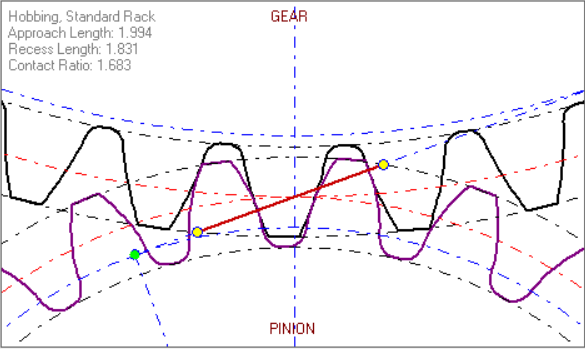
\includegraphics[width=0.75\textwidth]{figures/hip_gears.PNG}
    \end{figure}

    \null
    \vfill

\end{appendices}